\chapter{系統架構與規劃}
\label{c:intro}
本章介紹系統架構與佈局規劃。

\section{系統前半js與html之偵測} 
本研究欲建設一模擬的平台,在此使用者可以打字於一框內,此框能傳送使用者所打出的文字與計算時間的數據至往後的分析系統裡。\\\\
%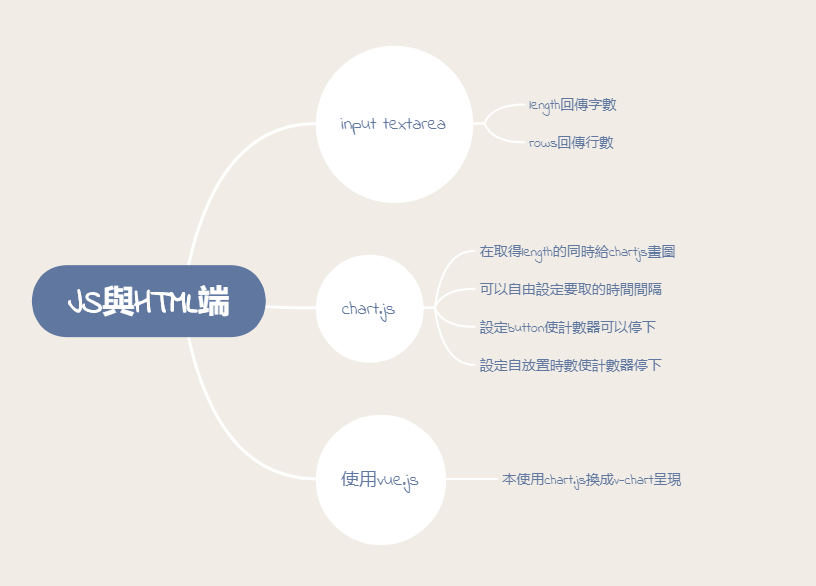
\includegraphics[width = .8\textwidth]{c5C4T4t.png}
\begin{figure}[H] %H为当前位置,!htb为忽略美学标准,htbp为浮动图形
		\centering %图片居中
		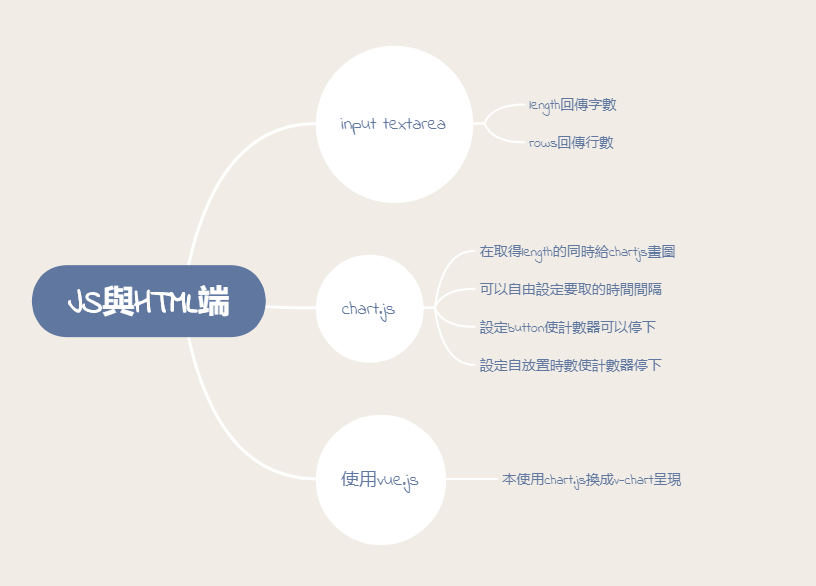
\includegraphics[width=0.7\textwidth]{c5C4T4t.png} %插入图片,[]中设置图片大小,{}中是图片文件名
		\caption{系統前半js與html架構} %最终文档中希望显示的图片标题
		\label{Fig.main2} %用于文内引用的标签
\end{figure}
\subsection{輸入}	
\begin{itemize}
	\item textarea的作用\\
	在html網頁中加上textarea的文字框,目的是建立一模擬的打字環境,畢竟本研究討論的是擷取使用者數據與分析其的重要;給使用者平台的管理並不在此研究範圍,因此使用最為簡單明瞭的文字框擷取。
\end{itemize}

\subsection{計算}
\begin{itemize}
	\item 字數與行數的判讀與計算\\
	擷取js程式:

\definecolor{lightgray}{rgb}{.9,.9,.9}
\definecolor{darkgray}{rgb}{.4,.4,.4}
\definecolor{purple}{rgb}{0.65, 0.12, 0.82}

\lstdefinelanguage{JavaScript}{
	keywords={typeof, new, true, false, catch, function, return, null, catch, switch, var, if, in, while, do, else, case, break},
	keywordstyle=\color{blue}\bfseries,
	ndkeywords={class, export, boolean, throw, implements, import, this},
	ndkeywordstyle=\color{darkgray}\bfseries,
	identifierstyle=\color{black},
	sensitive=false,
	comment=[l]{//},
	morecomment=[s]{/*}{*/},
	commentstyle=\color{purple}\ttfamily,
	stringstyle=\color{red}\ttfamily,
	morestring=[b]',
	morestring=[b]"
}

\lstset{
	language=JavaScript,
	backgroundcolor=\color{lightgray},
	extendedchars=true,
	basicstyle=\footnotesize\ttfamily,
	showstringspaces=false,
	showspaces=false,
	numbers=left,
	numberstyle=\footnotesize,
	numbersep=9pt,
	tabsize=2,
	breaklines=true,
	showtabs=false,
	captionpos=b
}

	\medskip
\begin{lstlisting}[caption=js字數與行數的判讀與計算]
function cal_words(){
	var length = document.getElementById("test").value.length;
   //獲取字數數量
	document.getElementById("num").innerHTML = length;
	//回傳給html並顯示
	var rows = document.getElementById("test").value.match(/\r?\n|\r/g).length;
	//抓取換行的字符個數
	document.getElementById("enter").innerHTML =rows;
	//回傳給html並顯示
}
\end{lstlisting}
在使用者打字在textarea時,可以使用javascript語法回傳在文字框的字行數據。
行數據的判斷方法有些許差異,在此我用的是只要使用者打自使用到換行,如enter字符,便會判斷為增加一行。
獲取這些數據後會回傳至html網頁顯示。
\item 時間的判讀與計算\\
我所使用的方法是setTimeout與setInterva函數,但是setTimeout函數只能循環一次,而setInterval()可以不斷循環,故使用setInterval更好。\cite{name20}
也就是說,我加上了固定秒數、時間的基礎上回傳字數資料,相當於固定的時間定時的收集textarea的數據;
如此一來,把時間與數據集中便可以知道時間與使用者打字的關係,進而能夠做到接下來分析的動作。

\end{itemize}
\subsection{輸出}
\begin{itemize}
	\item 圖表\\
	除了能夠獲取實質上的數據數字外,我使用了chart.js與vue.js進行數據繪圖與整理。\cite{name21}
	\begin{figure}[H] %H为当前位置,!htb为忽略美学标准,htbp为浮动图形
		\centering %图片居中
		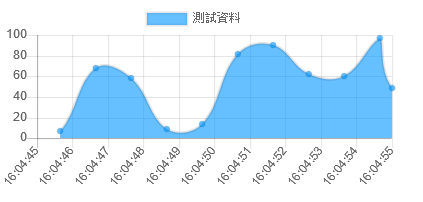
\includegraphics[width=0.7\textwidth]{3_1_3.png} %插入图片,[]中设置图片大小,{}中是图片文件名
		\caption{範例圖片} %最终文档中希望显示的图片标题
		\label{Fig.main2} %用于文内引用的标签
	\end{figure}
此範例圖片是每隔一段時間隨機取一數字並畫成圖,推送至html網頁,他是即時更新的圖表。
而在前頭所提及的setInterval()函數,可與圖表結合,可以更改setInterval()函數所選取的秒數擷取不同時間。所以圖表的輸出為: X軸時間,Y軸字數與行數
	\item 其他功能\\
	除及時推送的圖表外,另加入按鈕可使圖表停止推送。此動作相當於繳交,若要上繳自己所完成的文字檔必定儲存與離開本在工作的頁面,所以圖表與數據計算會停止不再更新與紀錄。
\end{itemize}
\section{系統後半colab分析部分}
	\begin{figure}[H] %H为当前位置,!htb为忽略美学标准,htbp为浮动图形
	\centering %图片居中
	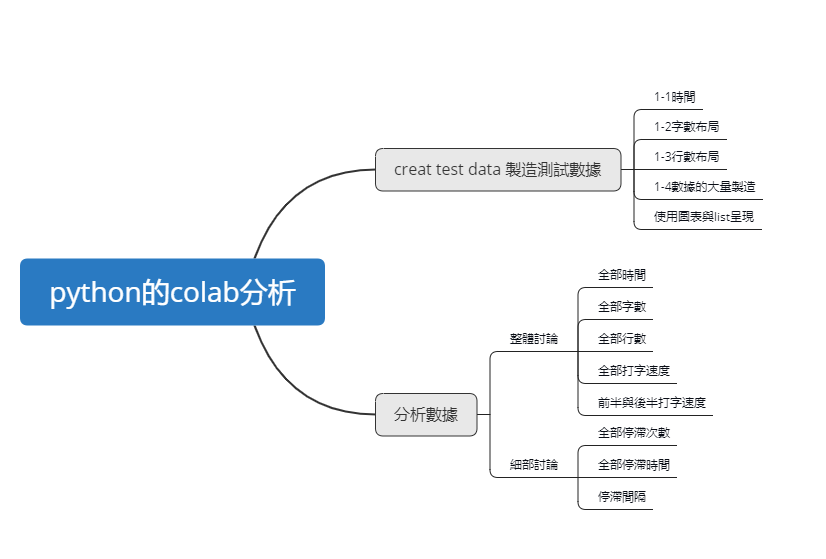
\includegraphics[width=0.7\textwidth]{3_2.png} %插入图片,[]中设置图片大小,{}中是图片文件名
	\caption{分析系統架構} %最终文档中希望显示的图片标题
	\label{Fig.main2} %用于文内引用的标签
\end{figure}